\textbf{Preventivo orario}

\begin{tblr}{
    colspec={|X[5cm]|X[.5cm]|X[.5cm]|X[.5cm]|X[.5cm]|X[.5cm]|X[.5cm]|X[3.5cm]},
    row{odd}={bg=white},
    row{even}={bg=lightgray},
    row{1}={bg=black, fg=white},
    row{8}={bg=black, fg=white}
}

    Nominativo & Re & Am & An & Pg & Pr & Vf & Ore Totali \\ \hline
    Alberto C. & - & - & 5 & - & - & - & 5 \\ \hline
    Bilal El M. & - & - & 5 & - & - & 7 & 12 \\ \hline
    Alberto M. & - & - & 10 & - & - & 2 & 12 \\ \hline
    Alex S. & - & 5 & 5 & - & - & - & 10 \\ \hline
    Iulius S. & - & - & 10 & - & - & 2 & 12 \\ \hline
    Giovanni Z. & 5 & - & - & - & - & - & 5 \\ \hline
    Totale & 5 & 5 & 35 & 0 & 0 & 11 & 56\\ \hline

\end{tblr}

\textbf{Preventivo economico}

\begin{tblr}{
colspec={|X[5cm]|X[3.5cm]|X[1.5cm]|X[3.5cm]},
row{odd}={bg=white},
row{even}={bg=lightgray},
row{1}={bg=black, fg=white},
row{8}={bg=black, fg=white}
}

Ruolo & Costo orario (€/h) & N. Ore & Costo totale (€) \\ \hline
Responsabile & 30,00 & 5 & 150,00 \\ \hline
Amministratore & 20,00 & 5 & 100,00 \\ \hline
Analista & 25,00 & 35 & 875,00 \\ \hline
Progettista & 25,00 & 0 & 0,00 \\ \hline
Programmatore & 15,00 & 0 & 0,00 \\ \hline
Verificatore & 15,00 & 11 & 165,00 \\ \hline
Totale & \SetCell[c=1]{c} & 56 & 1.290,00 \\ \hline

\end{tblr}
\pagebreak

\textbf{Attività svolte}

\paragraph{}
Le attività svolte dal gruppo nel terzo periodo sono state:
\begin{itemize}
    \item Stesura della prima versione dell'Analisi dei Requisiti;
    \item Inizio della stesura del Piano di Qualifica;
    \item Creazione di una script per la verifica automatica dell'aderenza dei documenti alle norme tipografiche indicate nelle Norme di Progetto;
    \item Prosieguo della stesura delle Norme di Progetto;
    \item Migrazione di tutta la documentazione dalla cartella presente su \emph{Google Drive}$^{G}$, alla repository su GitHub$^{G}$;
    \item Adozione di nuovi metodi per la gestione della configurazione dei documenti all'interno della repository, per una produzione più efficiente degli stessi da parte dei membri del gruppo;
    \item Incontro con il prof. Cardin nel quale è stato presentato il PoC e il documento di Analisi dei Requisiti.
\end{itemize}

\begin{figure}[H] 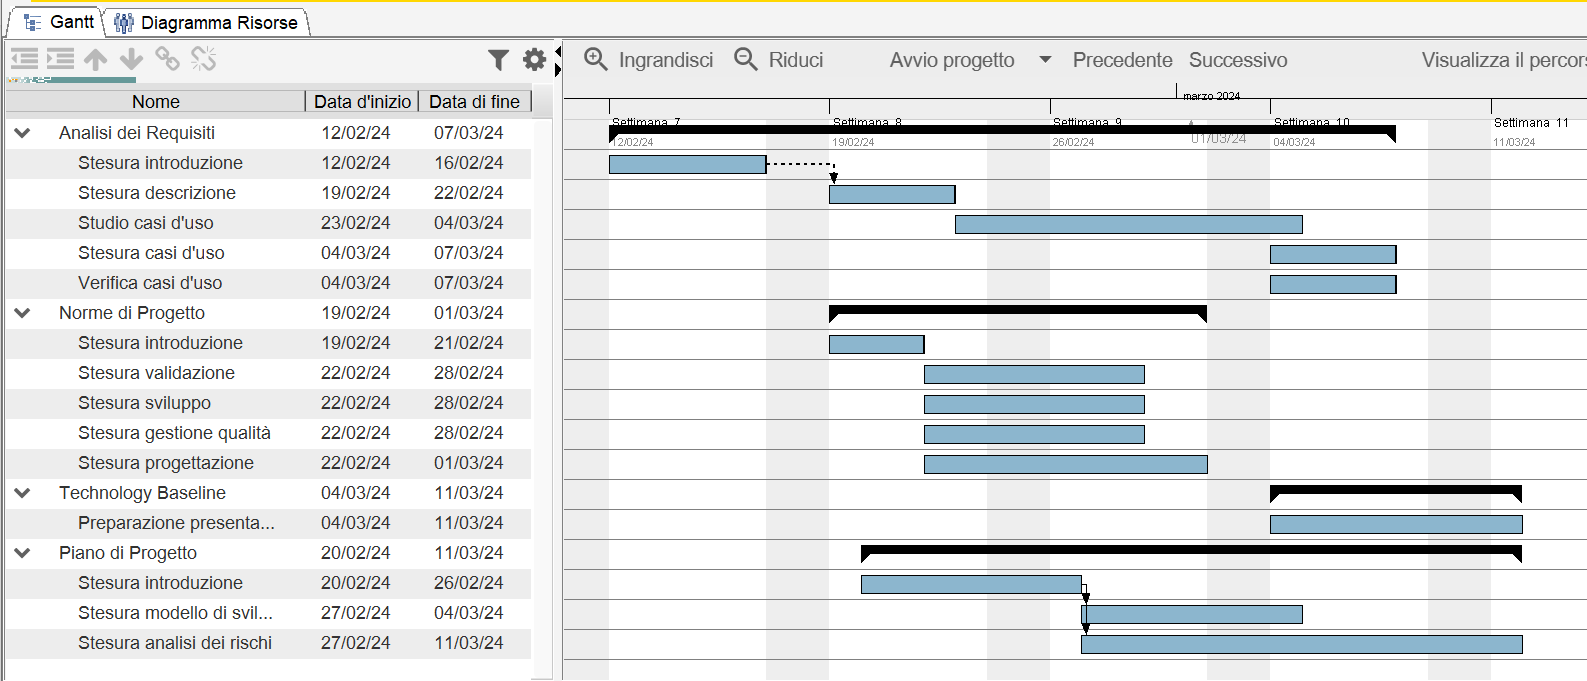
\includegraphics[scale=.6]{GanttTerzoPeriodo.png} \end{figure}


\textbf{Consuntivo orario}

\begin{tblr}{
    colspec={|X[5cm]|X[.5cm]|X[.5cm]|X[.5cm]|X[.5cm]|X[.5cm]|X[.5cm]|X[3.5cm]},
    row{odd}={bg=white},
    row{even}={bg=lightgray},
    row{1}={bg=black, fg=white},
    row{8}={bg=black, fg=white}
}

    Nominativo & Re & Am & An & Pg & Pr & Vf & Ore Totali \\ \hline
    Alberto C. & - & 2 & 3 & - & - & - & 5 \\ \hline
    Bilal El M. & - & - & 2 & - & - & 3 & 5 \\ \hline
    Alberto M. & - & - & 12 & - & - & 5 & 17 \\ \hline
    Alex S. & - & 5 & 10 & - & - & 5 & 20 \\ \hline
    Iulius S. & - & - & 12 & - & - & 5 & 17 \\ \hline
    Giovanni Z. & 5 & - & 3 & - & - & 2 & 10 \\ \hline
    Totale & 5 & 7 & 42 & 0 & 0 & 20 & 74 \\ \hline

\end{tblr}

\pagebreak
\textbf{Consuntivo economico}

\begin{tblr}{
colspec={|X[5cm]|X[3.5cm]|X[1.5cm]|X[3.5cm]},
row{odd}={bg=white},
row{even}={bg=lightgray},
row{1}={bg=black, fg=white},
row{8}={bg=black, fg=white}
}

Ruolo & Costo orario (€/h) & N. Ore & Costo totale (€) \\ \hline
Responsabile & 30,00 & 5 & 150,00 \\ \hline
Amministratore & 20,00 & 7 & 140,00 \\ \hline
Analista & 25,00 & 42 & 1050,00 \\ \hline
Progettista & 25,00 & 0 & 0,00 \\ \hline
Programmatore & 15,00 & 0 & 0,00 \\ \hline
Verificatore & 15,00 & 20 & 300,00 \\ \hline
Totale & \SetCell[c=1]{c} & 74 & 1.640,00 \\ \hline

\end{tblr}

\textbf{Gestione dei ruoli}

\paragraph{}
Nel terzo periodo, il 56\% delle risorse temporali del gruppo è stato speso nel ruolo dell'Analista, data la necessità
di portare a compimento la stesura della prima versione dell'Analisi dei Requisiti in vista della prima fase della revisione
RTB; di conseguenza il gruppo ha utilizzato il 27\% delle ore per i processi di verifica e validazione del documento sopra citato, processi che
sono stati visionati dai membri con particolare attenzione, vista l'importanza del documento stesso; inoltre il 9\% delle ore sono state dedicate alla figura dell'Amministratore
migrazione di tutta la documentazione sulla repository in GitHub e alla messa a punto della relativa gestione di configurazione, operazioni alle quali ha partecipato anche il Responsabile.



\paragraph{Gestione dei rischi}

\begin{itemize}
\item \textbf{Rischio verificatosi:} Analisi incompleta/carente dei requisiti:
\begin{itemize}
\item \textbf{Esito Piano di Contingenza:} I membri del gruppo deputati alla stesura dell'Analisi dei Requisiti hanno constatato tardivamente che i requisiti funzionali individuati prima del terzo periodo fossero insufficienti, in termini di numero e di profondità dell'analisi stessa; si è deciso quindi di destinare un maggior numero di ore a quest'ultima e di incrementare da 2 a 3 il numero di componenti deputati ad essa;
\item \textbf{Impatto:} Significativo è stato l'impatto del suddetto rischio, avendo comportato la necessità da parte del gruppo, di riallocare parte delle risorse orarie, dedicando 7 ore in più alla fase di analisi senza però aumentare il monte orario complessivo preventivato all'inizio del terzo periodo; sono state quindi tolte risorse alla stesura degli altri documenti.
\end{itemize}

\item \textbf{Rischio verificatosi:} Calcolo delle tempistiche:
\begin{itemize}
\item \textbf{Esito Piano di Contingenza:} In seguito al verificarsi del rischio legato ad una carente analisi dei requisiti, il Responsabile ha realizzato che sarebbe stato necessario aumentare non solo le ore da dedicare all'analisi stessa, ma anche alla verifica e validazione delle sezioni del relativo documento, che venivano iterativamente prodotte e corrette; il gruppo è riuscito a non aumentare il monte orario preventivato all'inizio del terzo periodo;
\item \textbf{Impatto:} L'impatto è stato significativo; nonostante non direttamente misurabile in un aumento del monte orario preventivato, si è tradotto in un'importante riallocazione di ore, tolte dal prosieguo della stesura della restante documentazione (in particolare del Piano di Qualifica).
\end{itemize}\pagebreak
\item \textbf{Rischio verificatosi:} Disponibilità dei membri:
\begin{itemize}
    \item \textbf{Esito Piano di Contingenza:} In concomitanza dell'inizio della sessione d'esami, non è stato possibile una redistribuzione dei compiti dai membri con un numero maggiore di esami da sostenere a quelli meno impegnati; di comune accordo si è deciso quindi di interrompere fino al termine della sessione le attività del gruppo;
    \item \textbf{Impatto:} L'impatto è stato importante in quanto vi è stato un rallentamento eccessivo da parte di tutti i membri del gruppo, nonostante esso fosse stato preventivato; tale impatto è misurabile in un ritardo di 14 giorni rispetto alla tabella di marcia.
\end{itemize}
\end{itemize}

\paragraph{}
\textbf{Retrospettiva:} \\
Nel terzo periodo, essendo stata completata la codifica del PoC, il gruppo ha speso la maggior parte delle proprie risorse per proseguire la stesura dei documenti, con attenzione
particolare nei confronti dell'Analisi dei Requisiti data la volontà di recuperare parte del ritardo accumulato sulla tabella di marcia e di voler effettuare la prima parte dell'RTB.\\
Purtroppo, come avvenuto nel secondo periodo, il ritmo di lavoro ha subito un nuovo rallentamento a causa della sessione invernale di esami, rendendo evidente da parte del gruppo una
parziale incapacità di mettere in atto un efficiente piano di contingenza con i rischi di una scarsa comunicazione e di una fallace pianificazione; data l'importanza dell'Analisi
dei Requisiti, si è reso necessario concentrare in essa buona parte delle risorse orarie, rallentando così la stesura degli altri documenti.
\begin{itemize}
    \item \textbf{Obbiettivi raggiunti:}
    \begin{itemize}
        \item Stesura della prima versione dell'Analisi dei Requisiti;
        \item Inizio della stesura del Piano di Qualifica;
        \item Inizio della stesura del Glossario;
        \item Prosieguo della stesura delle Norme e del Piano di Progetto;
        \item Creazione di uno script per la verifica automatica dei documenti.
    \end{itemize}
    \item \textbf{Obiettivi mancati:}
    \begin{itemize}
        \item Stesura della prima versione delle Norme di Progetto;
        \item Stesura della prima versione del Piano di Progetto.
    \end{itemize}
\end{itemize}
